\documentclass{article}
\usepackage{graphicx} % Required for inserting images
\usepackage[T2A]{fontenc}
\usepackage{titlesec}
%\usepackage{verbatim}
\usepackage[left=25mm, right=15mm, top=20mm, bottom=20mm, footskip=10mm]{geometry}
\usepackage{amsmath}
\usepackage{epigraph}
\usepackage{tikz}
\usepackage{latexsym}
%\usepackage{listings}
\frenchspacing 
\newcommand{\path}{\rightsquigarrow}
\titleformat{\section}[hang]{\normalsize\bfseries}{\thesection~}{0pt}{}
\titlespacing{\section}{\parindent}{\baselineskip}{\baselineskip}

\titleformat{\subsection}[hang]{\normalsize}{\thesubsection~}{0pt}{}
\titlespacing{\subsection}{\parindent}{0pt}{0pt}
\parindent=1.25cm 

\title{Тема 2. Обход в глубину. Связность неориентированных графов }
\date{}

\begin{document}

\maketitle

\epigraph{Автор конспекта: Родион Лыков}


\begin{center}
\includegraphics[scale=0.3]{image.png}

Это я пишу вам эту лекцию! 
\end{center}

\section{Основные термины}

\begin{enumerate}
\item \textit{Путь} в простом графе между двумя вершинами есть последовательность смежных вершин. Если между двумя вершинами $a,b$ существует путь, то обозначают это как $a \rightarrow b$.
Давайте рассмотрим некоторые свойства пути в неориентированном графе. 
\begin{enumerate}
    \item Свойство рефлексивности: $\forall a \in V : a \rightarrow a$. 
    \item Свойство симметричности: $\forall a,b \in V  : a \rightarrow b \Rightarrow b \rightarrow a$
    \item Свойство транзитивности: $\forall a,b,c \in V  : a \rightarrow b, b \rightarrow c \Rightarrow a \rightarrow c$
\end{enumerate}

\item \textit{Связным} называется неориентированный граф, для которого между любыми парами вершин существует путь. 
\item \textit{Компонентой связности} графа называется такое множество $S$ вершин, что между всеми вершинами в $S$ есть путь и нельзя добавить ни одну вершину в множество $S$, чтобы это свойство сохранялось. 
\item Если в графе \textit{одна компонентна связности}, то граф связный. 
\item \textit{Мостом} в графе называется такое ребро, что при его удалении количество компонент связности увеличится. 
\item \textit{Точкой сочленения} в графе называется такая вершина, что при ее удалении (удаляются также все ребра, инцидентные данной вершине) количество компонент связности увеличится.
\end{enumerate}

В следующем графе две компоненты связности, обозначил их разными цветами: 

\begin{center}
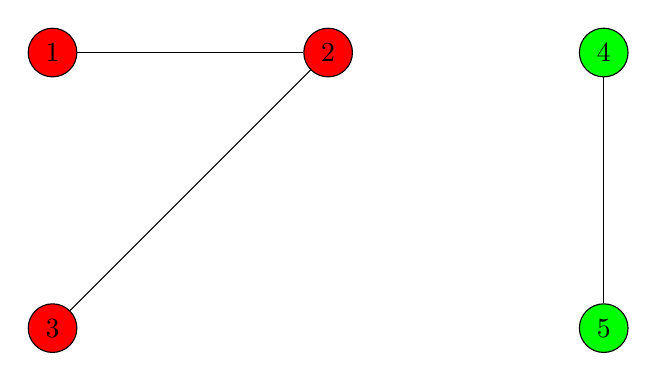
\begin{tikzpicture}[main/.style = {draw, circle},node distance={35mm}] 
\node[main] (1) [fill=red]{$1$}; 
\node[main] (2) [right of=1,fill=red] {$2$}; 
\node[main] (3) [below of=1,fill=red] {$3$};
\node[main] (4) [right of=2,fill=green] {$4$};
\node[main] (5) [below of=4,fill=green] {$5$};
\draw (1) -- (2);
\draw (2) -- (3);
\draw (4) -- (5);
\end{tikzpicture} 

\end{center}

Давайте, кстати, подумаем, как задать такой граф списком смежности: 

\begin{verbatim}
    e[1] = [2]
    e[2] = [1,3]
    e[3] = [2]
    e[4] = [5]
    e[5] = [4]
\end{verbatim}

\section{Алгоритм поиска в глубину}

Итак, давайте научимсярешать самую простую задачу: проверить, правда ли в графе есть путь между вершиной $a$ и вершиной $b$. Здесь познакомимся с алгоритмом <<Поиска в глубину>>, который применяется в большинстве задач на графы! Сам граф будем хранить списком смежности. 

Итак, алгоритм очень просто описать словами: пусть нам нужно найти путь из вершины $a$ в вершину $b$, тогда давайте начнем в вершине $a$ и пройдем по случайному ребру, по которому мы еще не проходили. Затем будем повторять процесс: идти по случайному ребру из текущей вершины, главное не посещать одну вершину более раза, чтобы не зациклить наш алгоритм.  

Давайте представим это все на примере, пусть нам дан такой граф:

\begin{center}
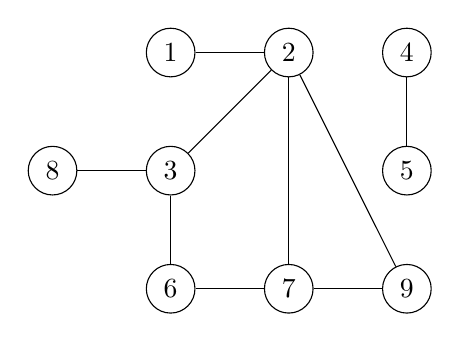
\begin{tikzpicture}[main/.style = {draw, circle},node distance={15mm}] 
\node[main] (1) []{$1$}; 
\node[main] (2) [right of=1] {$2$}; 
\node[main] (3) [below of=1] {$3$};
\node[main] (4) [right of=2] {$4$};
\node[main] (5) [below of=4] {$5$};
\node[main] (6) [below of=3] {$6$};
\node[main] (7) [right of=6] {$7$};
\node[main] (8) [left of=3] {$8$};
\node[main] (9) [right of=7] {$9$};
\draw (1) -- (2);
\draw (2) -- (3);
\draw (4) -- (5);
\draw (8) -- (3);
\draw (3) -- (6);
\draw (7) -- (6);
\draw (7) -- (2);
\draw (7) -- (9);
\draw (2) -- (9);
\end{tikzpicture} 

\end{center}

Рассмотрим, как будет проходить наш алгоритм (отметим красной вершиной ту, в которой мы сейчас находимся, а зелеными вершинами будем отмечать те, которые уже посетили). Будем каждый раз ходить по случайному ребру, главное не в зеленую вершину. Если ребер из текущей (красной) вершины нету, но вернемся в любую вершину, из которой мы еще не рассмотрели все ребра. Итак, ищем путь $1 \rightarrow 9$:

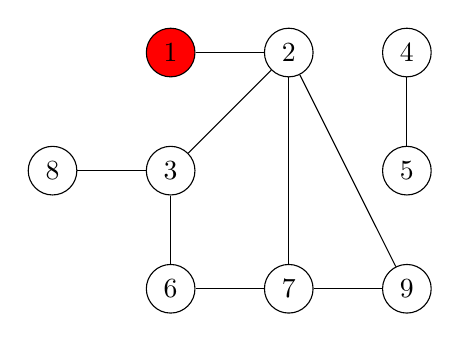
\begin{tikzpicture}[main/.style = {draw, circle},node distance={15mm}] 
\node[main] (1) [fill=red]{$1$}; 
\node[main] (2) [right of=1] {$2$}; 
\node[main] (3) [below of=1] {$3$};
\node[main] (4) [right of=2] {$4$};
\node[main] (5) [below of=4] {$5$};
\node[main] (6) [below of=3] {$6$};
\node[main] (7) [right of=6] {$7$};
\node[main] (8) [left of=3] {$8$};
\node[main] (9) [right of=7] {$9$};
\draw (1) -- (2);
\draw (2) -- (3);
\draw (4) -- (5);
\draw (8) -- (3);
\draw (3) -- (6);
\draw (7) -- (6);
\draw (7) -- (2);
\draw (7) -- (9);
\draw (2) -- (9);
\end{tikzpicture} 
\qquad 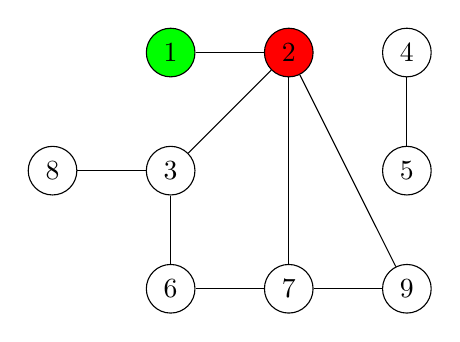
\begin{tikzpicture}[main/.style = {draw, circle},node distance={15mm}] 
\node[main] (1) [fill=green]{$1$}; 
\node[main] (2) [right of=1][fill=red] {$2$}; 
\node[main] (3) [below of=1] {$3$};
\node[main] (4) [right of=2] {$4$};
\node[main] (5) [below of=4] {$5$};
\node[main] (6) [below of=3] {$6$};
\node[main] (7) [right of=6] {$7$};
\node[main] (8) [left of=3] {$8$};
\node[main] (9) [right of=7] {$9$};
\draw (1) -- (2);
\draw (2) -- (3);
\draw (4) -- (5);
\draw (8) -- (3);
\draw (3) -- (6);
\draw (7) -- (6);
\draw (7) -- (2);
\draw (7) -- (9);
\draw (2) -- (9);
\end{tikzpicture} 
\newline \newline \newline
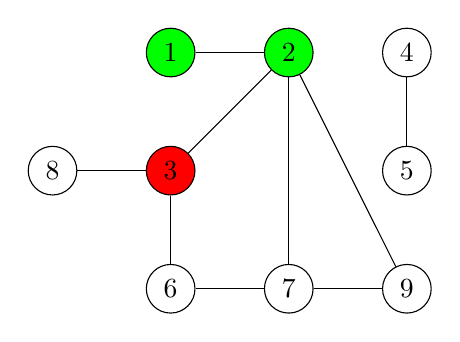
\begin{tikzpicture}[main/.style = {draw, circle},node distance={15mm}] 
\node[main] (1) [fill=green]{$1$}; 
\node[main] (2) [right of=1][fill=green] {$2$}; 
\node[main] (3) [below of=1][fill=red] {$3$};
\node[main] (4) [right of=2] {$4$};
\node[main] (5) [below of=4] {$5$};
\node[main] (6) [below of=3] {$6$};
\node[main] (7) [right of=6] {$7$};
\node[main] (8) [left of=3] {$8$};
\node[main] (9) [right of=7] {$9$};
\draw (1) -- (2);
\draw (2) -- (3);
\draw (4) -- (5);
\draw (8) -- (3);
\draw (3) -- (6);
\draw (7) -- (6);
\draw (7) -- (2);
\draw (7) -- (9);
\draw (2) -- (9);
\end{tikzpicture} 
\qquad 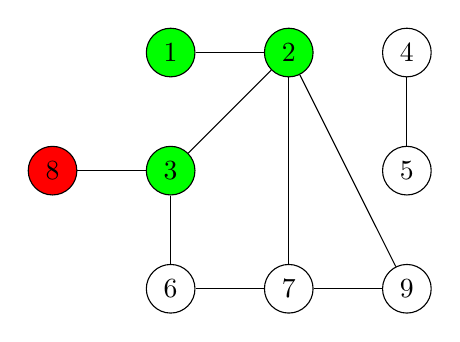
\begin{tikzpicture}[main/.style = {draw, circle},node distance={15mm}] 
\node[main] (1) [fill=green]{$1$}; 
\node[main] (2) [right of=1][fill=green] {$2$}; 
\node[main] (3) [below of=1][fill=green] {$3$};
\node[main] (4) [right of=2] {$4$};
\node[main] (5) [below of=4] {$5$};
\node[main] (6) [below of=3] {$6$};
\node[main] (7) [right of=6] {$7$};
\node[main] (8) [left of=3,fill=red] {$8$};
\node[main] (9) [right of=7] {$9$};
\draw (1) -- (2);
\draw (2) -- (3);
\draw (4) -- (5);
\draw (8) -- (3);
\draw (3) -- (6);
\draw (7) -- (6);
\draw (7) -- (2);
\draw (7) -- (9);
\draw (2) -- (9);
\end{tikzpicture} 
\newline \newline \newline
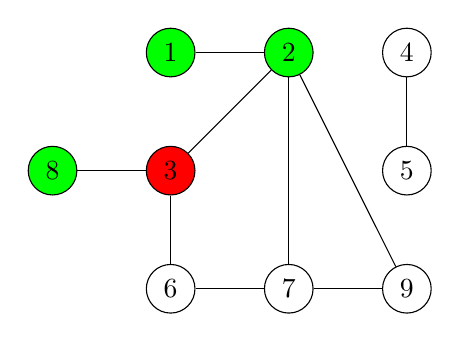
\begin{tikzpicture}[main/.style = {draw, circle},node distance={15mm}] 
\node[main] (1) [fill=green]{$1$}; 
\node[main] (2) [right of=1][fill=green] {$2$}; 
\node[main] (3) [below of=1][fill=red] {$3$};
\node[main] (4) [right of=2] {$4$};
\node[main] (5) [below of=4] {$5$};
\node[main] (6) [below of=3] {$6$};
\node[main] (7) [right of=6] {$7$};
\node[main] (8) [left of=3,fill=green] {$8$};
\node[main] (9) [right of=7] {$9$};
\draw (1) -- (2);
\draw (2) -- (3);
\draw (4) -- (5);
\draw (8) -- (3);
\draw (3) -- (6);
\draw (7) -- (6);
\draw (7) -- (2);
\draw (7) -- (9);
\draw (2) -- (9);
\end{tikzpicture} 
\qquad 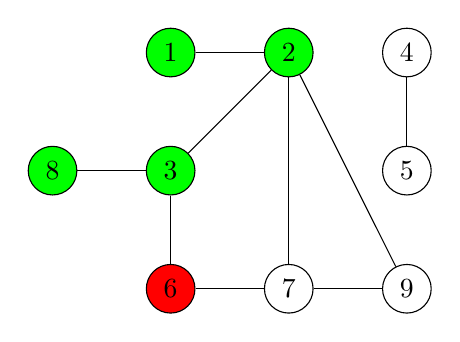
\begin{tikzpicture}[main/.style = {draw, circle},node distance={15mm}] 
\node[main] (1) [fill=green]{$1$}; 
\node[main] (2) [right of=1][fill=green] {$2$}; 
\node[main] (3) [below of=1][fill=green] {$3$};
\node[main] (4) [right of=2] {$4$};
\node[main] (5) [below of=4] {$5$};
\node[main] (6) [below of=3,fill=red] {$6$};
\node[main] (7) [right of=6] {$7$};
\node[main] (8) [left of=3,fill=green] {$8$};
\node[main] (9) [right of=7] {$9$};
\draw (1) -- (2);
\draw (2) -- (3);
\draw (4) -- (5);
\draw (8) -- (3);
\draw (3) -- (6);
\draw (7) -- (6);
\draw (7) -- (2);
\draw (7) -- (9);
\draw (2) -- (9);
\end{tikzpicture} 
% 1->2->3->6
\newline \newline \newline
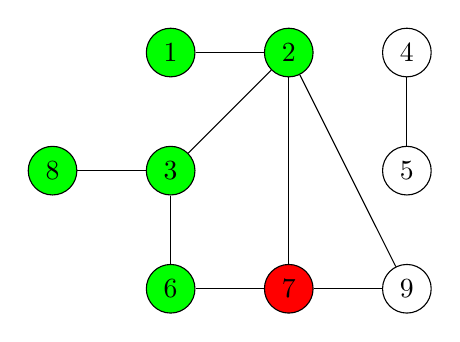
\begin{tikzpicture}[main/.style = {draw, circle},node distance={15mm}] 
\node[main] (1) [fill=green]{$1$}; 
\node[main] (2) [right of=1][fill=green] {$2$}; 
\node[main] (3) [below of=1][fill=green] {$3$};
\node[main] (4) [right of=2] {$4$};
\node[main] (5) [below of=4] {$5$};
\node[main] (6) [below of=3,fill=green] {$6$};
\node[main] (7) [right of=6,fill=red] {$7$};
\node[main] (8) [left of=3,fill=green] {$8$};
\node[main] (9) [right of=7] {$9$};
\draw (1) -- (2);
\draw (2) -- (3);
\draw (4) -- (5);
\draw (8) -- (3);
\draw (3) -- (6);
\draw (7) -- (6);
\draw (7) -- (2);
\draw (7) -- (9);
\draw (2) -- (9);
\end{tikzpicture} 
\qquad 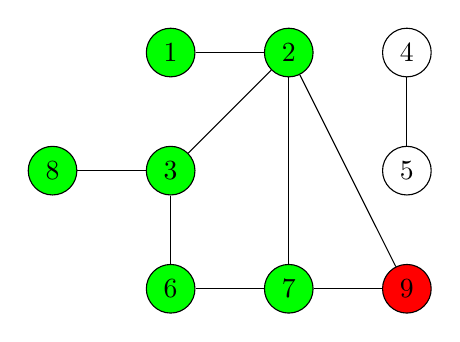
\begin{tikzpicture}[main/.style = {draw, circle},node distance={15mm}] 
\node[main] (1) [fill=green]{$1$}; 
\node[main] (2) [right of=1][fill=green] {$2$}; 
\node[main] (3) [below of=1][fill=green] {$3$};
\node[main] (4) [right of=2] {$4$};
\node[main] (5) [below of=4] {$5$};
\node[main] (6) [below of=3,fill=green] {$6$};
\node[main] (7) [right of=6,fill=green] {$7$};
\node[main] (8) [left of=3,fill=green] {$8$};
\node[main] (9) [right of=7,fill=red] {$9$};
\draw (1) -- (2);
\draw (2) -- (3);
\draw (4) -- (5);
\draw (8) -- (3);
\draw (3) -- (6);
\draw (7) -- (6);
\draw (7) -- (2);
\draw (7) -- (9);
\draw (2) -- (9);
\end{tikzpicture}  

Таким образом, мы достигли вершины $9$. Обратите внимание, раз мы выбираем любое ребро, то мы могли найти и другой путь, например: $1 \rightarrow 2 \rightarrow 9, 1 \rightarrow 2 \rightarrow 7 \rightarrow 9$. В принципе, нам не важен сам путь, нам важно лишь его наличие. Итак, напишем это в коде. Граф будем считывать в виде списка ребер, где сначала считаем количество вершин в графе, потом --- количество ребер. Будем обозначать $color_x = 0$, если вершина $x$ еще не посещена, и $color_x = 1$, если вершину $x$ мы в какой-то момент посетили. Очевидно, если мы посетим конечную вершину, то до нее есть путь. 

\section{Решения задач}

Приведем решение задачи: <<можно ли дойти из вершины $S$ в вершину $T$>>:

\begin{verbatim}
    #include <bits/stdc++.h>
    using namespace std;
    vector<int>color; 
    vector<vector<int>>e;
    int n,m;
    void dfs(int x) {
        if(color[x]) return;
        color[x] = 1;
        for(auto& y : e[x]) { // перебираем любое ребро из вершины x
            dfs(y);
        }
    }
    void solve() {
        int S,T;
        cin >> S >> T;
        dfs(S);
        if(color[T]) {
            cout << "Yes\n";
        } else {
            cout << "No\n";
        }
    }
    int main() {
        cin >> n >> m;
        color = vector<int>(n+1);
        e = vector<vector<int>>(n+1);
        for(int i = 1; i <= m; i++) {
            int x,y;
            cin >> x >> y;
            e[x].push_back(y);
            e[y].push_back(x);
        }
        solve();
    }
\end{verbatim}

Давайте еще раз отдельно посмотрим на основную часть алгоритма:

\begin{verbatim}
    vector<int>color; 
    void dfs(int x) { 
        if(color[x]) return; // если вершина уже посещена, выходим
        color[x] = 1; // помечаем вершину
        for(auto& y : e[x]) { // перебираем любое ребро из вершины x
            dfs(y); // идем по найденному ребру, запускаем тот же алгоритм
        }
    }
\end{verbatim}
Как вы можете заметить, здесь мы используем <<рекурсию>>, когда функция вызывает сама себя. В принципе, это мы и описали словами: выбрать любое ребро из вершины, перейти по этому ребру и повторить данный алгоритм. Условие if(color[x]) говорит о том, что данную вершину мы уже покрасили.

Здесь видно, что алгоритм работает за $O(n + m)$, так как мы один раз перебирем каждую вершину и два раза каждое ребро (из обоих его концов). 

Давайте поймем, как использовать алгоритм для решения следующей задачи: узнать, правда ли граф связный. Конечно, можно решить задачу за $O(n^2 (n+m))$: перебрать пару вершин $(a,b)$ за $O(n^2)$, затем за $O(n+m)$ проверить, есть ли путь из $a$ в $b$. Но вспоминайте транзитивное свойство пути: если из $a$ есть путь в $b$, а из $b$ есть путь в $c$, то есть путь из $a$ в $c$. Тогда, давайте найдем все достижимые вершины из вершины $a$. Если граф неориентированный, то мы посетим абсолютно все вершины графа. Если граф связный, то все вершины будут покрашены. Вершину $a$ можно выбрать абсолютно любой. Приведем реализацию: 

\begin{verbatim}
    #include <bists/stdc++.h>
    using namespace std;
    vector<int>color; 
    vector<vector<int>>e;
    int n,m;
    void dfs(int x) {
        if(color[x]) return;
        color[x] = 1;
        for(auto& y : e[x]) { // перебираем любое ребро из вершины x
            dfs(y);
        }
    }
    void solve() {
        dfs(1); // Запустим алгоритм поиска в глубину
        bool flag = 1;
        for(int i = 1; i <= n; i++) {
            if(color[i] == 0) {
                flag = 0; // нашли недостижимую вершину
            }
        }
        if(flag) {
            cout << "Connected\n"; // Связный!
        } else {
            cout << "Not connected\n"; // Видение: несвязный...
        }
    }
    int main() {
        cin >> n >> m;
        color = vector<int>(n+1);
        e = vector<vector<int>>(n+1);
        for(int i = 1; i <= m; i++) {
            int x,y;
            cin >> x >> y;
            e[x].push_back(y);
            e[y].push_back(x);
        }
        solve();
    }
\end{verbatim}

Конечно, алгоритм поиска в глубину можно использовать и для решения самых различных задач, будем их разбирать в следующих темах. Пока что продолжим решать задачи на пути: у нас есть граф, в котором все вершины названы различными словами (а не числами). Задача состоит в том, чтобы $q (q \leq 10)$ раз решить задачу: задается два целых числа $a,b$. Правда ли есть путь из $a$ в $b$. 
Например:

\begin{verbatim}
2 --- Это количество ребер графа
Ivan Dima // Это ребра
Misha Svyatoslav
3 // Это количество пар, для которых надо сказать ответ
Ivan Svyatoslav
Ivan Dima
Svyatoslav Misha
\end{verbatim}

Запомните: мы всегда работаем с графами, где вершины заданы целыми числами (или набором целых чисел), работать со словами сложно и неудобно. Итак, давайте для начала перенумеруем вершины! Заметьте, в этой задаче количество ребер $m$ не больше $3 \cdot 10^5$, тогда количество вершин не больше $2m$. Итак, у нас будет функция $num$, которая принимает строку и возвращает ее номер. То есть мы присвоим каждому имени свое уникальное число:

\begin{verbatim}
//Только сначала глобальные переменные!
const int MAX = 600'000 + 10; // кол-во вершин
vector<vector<int>>e;
vector<int>color;
\end{verbatim}

\begin{verbatim}
int K = 0;
map<string,int>_num;
int num(string s) {
    if(_num.find(s) == _num.end()) { // еще не пронумеровано
        K++;
        _num[s] = K; // нумеруем новым числом K, заметьте, что мы его увеличили на 1
        return K;
    }
    return _num[s];
}
\end{verbatim}

Теперь давайте посмотрим, как будет выглядеть main():

\begin{verbatim}
int main() {
    ios::sync_with_stdio(0);
    cin.tie(0);
    cout.tie(0); // делаем быстрый ввод-вывод
    int m;
    cin >> m;
    color = vector<int>(MAX+1);
    e = vector<vector<int>>(MAX+1);
    for(int i = 1; i <= m; i++) {
        string a,b;
        cin >> a >> b; 
        int x = num(a);
        int y = num(b);
        e[x].push_back(y);
        e[y].push_back(x);
    }
    //Теперь граф готов, можем решать задачу!
}
\end{verbatim}

Задачу будем решать в функции solve(), но сначала допишем main() (добавим ввод очередной пары)

\begin{verbatim}
int main() {
    ios::sync_with_stdio(0);
    cin.tie(0);
    cout.tie(0); // делаем быстрый ввод-вывод
    int m;
    cin >> m;
    color = vector<int>(MAX+1);
    e = vector<vector<int>>(MAX+1);
    for(int i = 1; i <= m; i++) {
        string a,b;
        cin >> a >> b; 
        int x = num(a);
        int y = num(b);
        e[x].push_back(y);
        e[y].push_back(x);
    }
    int q;
    cin >> q;
    for(int i = 1; i <= q; i++) {
        string a,b;
        cin >> a >> b;
        int x = num(a);
        int y = num(b);
        solve(x,y);
    }   
}
\end{verbatim}

Теперь напишем функцию solve(), которая принимает пару вершин --- между которыми надо найти ответ.

\begin{verbatim}
void solve(int x, int y) {
    color = vector<int>(MAX+1); // А надо ли обнулять color? 
    dfs(x);
    if(color[y]) {
        cout << "Yes\n";
    } else {
        cout << "No\n";
    }
}
\end{verbatim}

Получим решение за $O(m \log{m} + n + m)$. Данный метод перенумерования графа всегда встречается, когда граф нам задан как-то неявно. 


\end{document}
